\chapter{波、量子化模式与产生算符}

\section{波、场与复指数}

量子场论是粒子物理学的基本工具。在哪怕只是初步介绍量子场之前，先汇集把波与粒子联系起来的数学事实是有益的。波本身已经是一种场构型：场在空间中逐点变化，而波就是那些值振荡并传播的一种构型。量子力学提供了这种波与粒子之间的联系。

这里假定读者已具备量子力学与狭义相对论的基础。当前的目的只是回顾粒子物理学所需的各个部分，而不是取代这两门学科中任何一门的课程。

指数函数的特征在于按比例增长。若
\begin{equation}
f(x)=e^{\alpha x},
\end{equation}
则
\begin{equation}
\frac{df}{dx}=\alpha f.
\end{equation}
在很小的区间内，增量与已经存在的量成正比。培养皿中增长的种群给出了熟悉的图景：存在的个体越多，可供繁殖的个体就越多，因此增长率与种群本身成正比。将\(e^{\alpha x}\)乘以一个整体常数并不改变这一定义性质。

正弦与余弦则振荡而不增长。它们是同一条曲线平移四分之一个周期，求导使它们相互旋转：
\begin{align}
\frac{d}{dx}\sin(kx)&=k\cos(kx),\\
\frac{d}{dx}\cos(kx)&=-k\sin(kx).
\end{align}
单独任何一个函数都不是指数函数，因为其导数与另一个函数成正比。而复组合确实具有指数性质。取\(i^2=-1\)，
\begin{align}
\frac{d}{dx}\bigl(\cos(kx)+i\sin(kx)\bigr)
&=-k\sin(kx)+ik\cos(kx)\\
&=ik\bigl(\cos(kx)+i\sin(kx)\bigr).
\end{align}
因此
\begin{equation}
e^{ikx}=\cos(kx)+i\sin(kx).
\end{equation}
这个恒等式反复出现，因为正弦和余弦描述类波的振荡。当\(x\)是空间坐标时，该函数在空间中振荡。当自变量是时间时，它在时间中振荡。

\section{频率、波长与光子动量}

普通频率\(f\)是每秒完整周期的数目。一个周期意味着一次完整振荡。角频率以弧度每秒度量同样的运动：
\begin{equation}
\omega=2\pi f.
\end{equation}
这两种记号描述的是同一个频率。人们在其中转换，是为了在计算中避免不必要的\(2\pi\)因子，尽管这些因子绝不会完全消失。

波长\(\lambda\)是一个完整空间周期所占据的距离。若波以速率\(v\)传播，则每周期距离乘以每秒周期数就是传播速率：
\begin{equation}
\lambda f=v.
\end{equation}
对于真空中的光，\(v=c\)，所以
\begin{equation}
\lambda f=c.
\end{equation}
对于声波，右端是声速；对于水波，它是相应的水波速率。因此\(c\)的出现是关于光的陈述，而不是对所有波都通用的定义。

量子力学以两种记号引入普朗克常数，
\begin{equation}
\hbar=\frac{h}{2\pi}.
\end{equation}
从\(h\)改为\(\hbar\)只是把\(2\pi\)因子从一个方程移到另一个方程。

有量纲常数的数值取决于用来表示它们的单位。米、秒和千克是人类尺度的约定，便于描述普通的长度和时间。与手臂长度相当的传统单位对布料或绳索很有用；无论通向米的历史路径具体如何，没有任何基本原理选择这一特定的人类尺度。在SI单位中，
\begin{equation}
\begin{aligned}
h &\simeq 6.6\times10^{-34}\ \mathrm{J\,s},
&\hbar &\simeq 1.1\times10^{-34}\ \mathrm{J\,s},\\
c &\simeq 3\times10^8\ \mathrm{m\,s^{-1}}.
\end{aligned}
\end{equation}
这些数字的意义在于它们在常规单位中的尺度：普朗克常数极其小，而光速极其大。

一个模式的一个量子具有能量
\begin{equation}
E_{\text{one quantum}}=\hbar\omega=hf.
\end{equation}
这是一个光子的能量，而不是任意经典电磁波的总能量。可见光的频率约为每秒\(10^{15}\)个周期，因此典型的光学光子能量约为
\begin{equation}
E_\gamma\sim 10^{-19}\ \mathrm{J}.
\end{equation}
即使如此快速的光学振荡，每个量子给出的能量也非常小，因为\(h\)如此之小。因此宏观量的光学能量包含数量巨大的光子。

能量和动量值得特别注意，因为二者都守恒。它们是有用的记账量：进入一个过程的总能量和动量必须与离开它的总能量和动量相平衡。动量是矢量，指向运动方向。对于运动远慢于光的粒子，
\begin{equation}
\vec p=m\vec v.
\end{equation}

现在考虑沿一个方向准直传播、而不是向许多方向发散的电磁辐射。它的动量指向束流方向。非相对论公式不能应用于光子，因为\(m\)表示静止质量，而光子的静止质量为零。尽管如此，仍有一个有用的量纲助记法。如果某人\emph{不恰当地}把量\(E/c^2\)当作质量赋予光子，然后代入\(v=c\)，就会得到
\begin{equation}
mv\longrightarrow \frac{E}{c^2}c=\frac{E}{c}.
\end{equation}
这一操作恰好给出正确答案，单位也正确，但它并不是光子具有静止质量\(E/c^2\)的正当论证。对于准直辐射，实际的相对论表述是
\begin{equation}
|\vec p|=\frac{E}{c}.
\end{equation}
该方程给出大小。方向就是辐射传播的方向。

对于一个光子，
\begin{align}
|\vec p_\gamma|
&=\frac{E_\gamma}{c}
=\frac{hf}{c}.
\end{align}
对于光，
\begin{equation}
\lambda f=c,
\qquad
\frac{f}{c}=\frac{1}{\lambda},
\end{equation}
因此
\begin{equation}
|\vec p_\gamma|=\frac{hf}{c}=\frac{h}{\lambda}.
\end{equation}

\begin{figure}[t]
\centering
\includegraphics[width=0.56\textwidth]{lecture_02_figure_02.png}
\caption{对于光，\(\lambda f=c\)和\(f/c=1/\lambda\)，即用于得到\(|\vec p_\gamma|=h/\lambda\)的关系。}
\lectureframe{00:21:39}
\end{figure}

波长越短，光子动量越大。这是粒子物理学中最重要的量子事实之一。要研究一个小物体，就需要短波长的探针，而这一短波长的代价就是大动量。

\begin{classroomqa}
\lecturetimestamp{00:22:23}
\audiencequestion{\(E=\hbar\omega\)是基本的，还是由更深层的原理推导出来的？}
\lecturerresponse{它由谐振子的量子力学推出。这里将直接使用这一结果，不再重复其证明；下文发展的振子语言为它提供了更深的背景。}
\end{classroomqa}


\section{波振幅与光子数}

\begin{classroomqa}
\lecturetimestamp{00:23:10}
\audiencequestion{用光子的语言来说，波的振幅意味着什么？}
\lecturerresponse{比较两个波长和频率相同但振幅不同的波，例如\(\sin(kx)\)和\(A\sin(kx)\)。经典地，固定区域内的能量正比于振幅的平方。量子力学地，包含\(n\)个光子的模式具有能量\(n\hbar\omega\)。在频率、区域和归一化固定时，振幅因此在数量级上按\(\sqrt n\)增长。}
\end{classroomqa}

这两个波的振荡图样完全相同。只是一个比另一个更强。\footnote{该示意图对应00处的波比较：23：47--00：24：28。}

\begin{figure}[t]
\centering
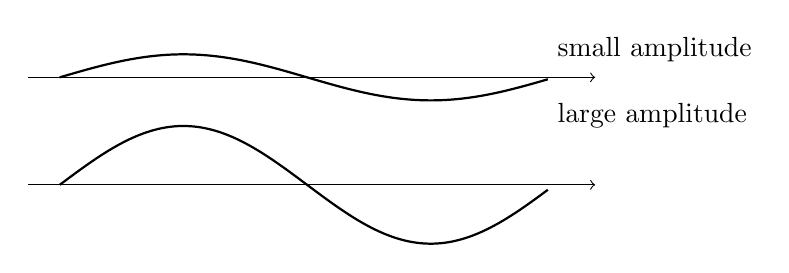
\begin{tikzpicture}[x=1cm,y=0.65cm]
\draw[->] (-0.4,0) -- (6.8,0);
\draw[->] (-0.4,-2.1) -- (6.8,-2.1);
\draw[thick] plot[domain=0:6.2,samples=120] (\x,{0.45*sin(\x r)});
\draw[thick] plot[domain=0:6.2,samples=120] (\x,{-2.1+1.15*sin(\x r)});
\draw (6.2,0.55) node[right]{small amplitude};
\draw (6.2,-0.75) node[right]{large amplitude};
\end{tikzpicture}
\caption{波长和频率相同但振幅不同的波。}
\end{figure}

对于固定数量的波，
\begin{equation}
E_{\text{wave}}\propto A^2.
\end{equation}
对于电磁波，这就是熟悉的陈述：场能正比于场强的平方。如果同一模式包含\(n\)个光子，那么
\begin{equation}
E_{\text{wave}}=n\hbar\omega.
\end{equation}
因此，在模式、频率、归一化和区域保持固定时，
\begin{equation}
A^2\propto n\hbar\omega,
\qquad
A\propto\sqrt n\quad\text{at fixed }\omega.
\end{equation}
这里并未断言任何精确的归一化。所包含的波的数量很重要：把原本均匀的波的长度加倍，会改变其总能量，而不改变局部振幅。因此，这一正比关系可以理解为对固定区域而言，例如一个波长。

还有一个量子特有的限定。振幅和相位不能同时被赋予精确的经典值。因此，问题``一个光子的振幅是多少？''如果要求一个完全锐利的经典场，就是含糊的。不过，令\(n=1\)仍给出一个合理的数量级尺度。

\begin{classroomqa}
\lecturetimestamp{00:28:25}
\audiencequestion{电磁波图中的竖直位移是否代表光子在空间中的位置？}
\lecturerresponse{不是。传播轴是空间的，而竖直坐标代表电场或磁场的值。动量沿传播轴方向，而不是沿所绘制的场振幅方向。}
\end{classroomqa}

波可以沿任意空间方向传播，但熟悉的 sinusoidal 图只把它的水平轴用作空间坐标。另一个绘制的方向记录场强。

\begin{classroomqa}
\lecturetimestamp{00:29:37}
\audiencequestion{所说的光子数是在一个波长或一个周期内计数的吗？}
\lecturerresponse{可以选择一个固定区域，例如一个波长。这就是为什么该关系只是正比关系：总能量和光子数还取决于包含了多少波。在相同振幅下，两个、三个或四个波长包含相应更多的能量。}
\end{classroomqa}

\begin{classroomqa}
\lecturetimestamp{00:30:17}
\audiencequestion{单个光子的振幅没有意义吗？}
\lecturerresponse{它只有在设定\(n=1\)后作为数量级陈述时才有意义。对于一个电磁模式，电场和磁场信息所起的作用类似于共轭的位置和动量信息，因此量子不确定性限制了经典振幅能被指定得多么精确。数量级关系仍然有用。}
\end{classroomqa}

这些问题已经引向量子场论，在那里场变量与粒子数之间的关系可以被精确陈述。目前这些比例关系已经足够。

\section{一般量子关系与慢物质波}

为光子引入的一些公式要普遍得多地适用，而另一些则不然。在转向电子之前，值得把它们分类整理。

\begin{figure}[t]
\centering
\includegraphics[width=0.82\textwidth]{lecture_02_figure_03.png}
\caption{波的定义以及光子和非相对论动量关系按其有效域进行比较。}
\lectureframe{00:31:52}
\end{figure}

\(f\)、\(\omega=2\pi f\)和\(\lambda\)的定义普遍适用。量子关系
\begin{equation}
E=\hbar\omega=hf
\end{equation}
在目前的讨论中也是普遍的。相比之下，含有\(c\)的公式，例如\(\lambda f=c\)和\(|\vec p|=E/c\)，适用于以光速运动的波。公式\(\vec p=m\vec v\)适用于运动远慢于光的粒子。介于这些极限之间的相对论运动需要一种目前还不需要的插值。

动量--波长关系在光子例子之后仍然成立：
\begin{equation}
p=\frac{h}{\lambda}.
\end{equation}
这里\(p\)表示当\(\lambda\)取为正波长时的大小；方向可以单独给出。

\begin{figure}[t]
\centering
\includegraphics[width=0.74\textwidth]{lecture_02_figure_04.png}
\caption{光子动量\(|\vec p_\gamma|=hf/c=h/\lambda\)，导致一般的德布罗意关系。}
\lectureframe{00:33:32}
\end{figure}

电子、原子核，甚至保龄球都可以与一个波相联系。电子干涉就是这一事实的一种表现。把电子波写成\(\psi\)。对于缓慢运动的电子，什么取代了\(\lambda f=c\)？缺失的成分是能量与动量之间的非相对论关系。

从动能和动量开始：
\begin{align}
E&=\frac12 mv^2,\\
p&=mv,
\qquad
v=\frac{p}{m}.
\end{align}
把最后一个关系代入第一个，得到
\begin{align}
E
&=\frac12m\left(\frac{p}{m}\right)^2\\
&=\frac{p^2}{2m}.
\end{align}
质量在\(\frac12 mv^2\)中位于分子，在\(p^2/(2m)\)中位于分母。这种位置很容易混淆，也值得重新推导。

现在使用一般量子关系
\begin{equation}
E=hf,
\qquad
p=\frac{h}{\lambda}.
\end{equation}
对于单个慢粒子，
\begin{align}
hf
&=\frac{p^2}{2m}\\
&=\frac{1}{2m}\left(\frac{h}{\lambda}\right)^2\\
&=\frac{h^2}{2m\lambda^2}.
\end{align}
除以\(h\)得到
\begin{equation}
f=\frac{h}{2m\lambda^2}.
\end{equation}

\begin{figure}[t]
\centering
\includegraphics[width=0.64\textwidth]{lecture_02_figure_05.png}
\caption{对于慢粒子，\(E=p^2/(2m)\)和\(p=h/\lambda\)给出\(f=h/(2m\lambda^2)\)。}
\lectureframe{00:37:47}
\end{figure}

对于光，
\begin{equation}
f\propto\frac{1}{\lambda},
\end{equation}
而对于慢物质，
\begin{equation}
f\propto\frac{1}{\lambda^2}.
\end{equation}
没有必要孤立地记住第二个关系。它总是可以从\(E=p^2/(2m)\)、\(E=hf\)和\(p=h/\lambda\)重建出来。对于在原子中缓慢运动的电子，它给出相应的Schr\"odinger波的频率。

\begin{classroomqa}
\lecturetimestamp{00:38:35}
\audiencequestion{非相对论频率--波长关系适用于电子以外的粒子吗？}
\lecturerresponse{是的。它适用于任何运动远慢于光的粒子。慢极限与类光极限之间的相对论插值是一个单独的主题。}
\end{classroomqa}

\begin{classroomqa}
\lecturetimestamp{00:38:55}
\audiencequestion{哪个关系适用于中微子？}
\lecturerresponse{这取决于中微子的速度。自然界中遇到的大多数中微子运动得非常接近光速，因此类光关系是一个很好的近似。运动远慢于光的中微子则会遵循非相对论关系。}
\end{classroomqa}

\editorialnote{在中微子问题之后紧接着有一段简短的听众交流，涉及振幅、量子和不同的电子波长，但其措辞损坏过重，无法可靠恢复。可恢复的回应推迟了不同波长的振幅与量子之间的一般关系。}

\begin{classroomqa}
\lecturetimestamp{00:39:56}
\audiencequestion{来自\(20\,\mathrm{keV}\)加速器的电子是慢的还是相对论的？}
\lecturerresponse{它被当作慢的来处理。在\(c=1\)的单位制中，质量、能量和动量可以用相同的单位表示。电子静能标度大致为\(0.5\,\mathrm{MeV}\)，而\(20\,\mathrm{keV}\)要小得多。等价地，非相对论动量判据是\(p\ll mc\)。}
\end{classroomqa}

例子中的能量比较为
\begin{equation}
K=20\,\mathrm{keV}\ll m_ec^2\simeq0.5\,\mathrm{MeV}.
\end{equation}
\editorialnote{ 00 处的源段落：39：56--00：41：40 将 \(20\,\mathrm{keV}\) 作为加速器能量引入，然后以动量与静质量的比较来表述相对论性判据。将动能判据和动量判据分别写出，既避免了把所引用的能量等同于动量，又保留了所述的非相对论性结论。}

\section{相速度、群速度与色散}

\begin{classroomqa}
\lecturetimestamp{00:41:46}
\audiencequestion{能否用频率乘以波长来得到电子波的速度？}
\lecturerresponse{它给出的是相速度，而不是赋予电子的速度。一个局域化的波包既有相速度，描述其内部波峰和波谷的运动，又有群速度，描述包络的运动。群速度被等同于粒子的运动。}
\end{classroomqa}

波包局部看起来像正弦或余弦，但被包络所限制。当它运动时，包络和其中的波峰不必以相同的速度运动。\footnote{该示意图依据 00 处的波包讨论：42：34--00：44：11。}

\begin{figure}[t]
\centering
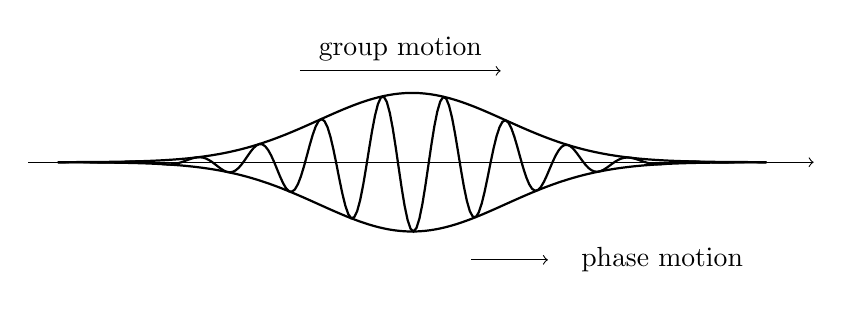
\begin{tikzpicture}[x=0.75cm,y=0.8cm]
\draw[->] (-0.5,0) -- (12.8,0);
\draw[thick] plot[domain=0:12,samples=140] (\x,{1.10*exp(-0.20*(\x-6)^2)});
\draw[thick] plot[domain=0:12,samples=140] (\x,{-1.10*exp(-0.20*(\x-6)^2)});
\draw[thick] plot[domain=0:12,samples=240] (\x,{1.10*exp(-0.20*(\x-6)^2)*sin(6*\x r)});
\draw[->] (4.1,1.45) -- (7.5,1.45);
\draw (5.8,1.8) node{group motion};
\draw[->] (7.0,-1.55) -- (8.3,-1.55);
\draw (8.7,-1.55) node[right]{phase motion};
\end{tikzpicture}
\caption{一个局域化的波包，其包络和内部相位通常以不同的速度运动。}
\end{figure}

相速度是单色成分的波峰、波谷及其他固定相位的速度。对于非相对论性色散关系，
\begin{equation}
v_\phi=f\lambda=\frac{h}{2m\lambda}.
\end{equation}
它依赖于波长。因此不同波长成分具有不同的相速度，所以波峰可以在波包中移动，波包可以发生色散。群速度是波包作为一个整体的速度，并且正是被等同于粒子的那个速度。

有一个简单的特例。如果所有波长成分都以相同的速度运动，相速度和群速度就一致。真空中的光具有这一性质：每一种波长都以 \(c\) 传播。慢粒子关系则不然；其 \(f\lambda\) 随 \(\lambda\) 变化。

方程
\begin{equation}
f=\frac{h}{2m\lambda^2}
\end{equation}
是自由 Schr\"odinger 方程的一种稍加伪装的形式。频率规定了平面波的时间依赖性，波长规定了其空间依赖性，而 Schr\"odinger 方程将二者联系起来。反过来，将具有确定频率、确定波长的波代入自由 Schr\"odinger 方程，会重现这一色散关系。

\begin{classroomqa}
\lecturetimestamp{00:47:02}
\audiencequestion{相速度能否超过光速？}
\lecturerresponse{能。相速度不携带信息。信息和局域化的波包以群速度传播，因此超光速的相速度并不允许超光速信号传递。}
\end{classroomqa}

\section{有限空间与离散动量}

最终关注的是无限空间中的波，但有限系统是更稳妥的出发点。无限不是计算机能够直接存储或操作的东西。人们先为有限系统建立方程，然后才取系统尺寸变为任意大的极限。这一习惯在整个量子力学、量子场论和粒子物理学中都有用。

从一维空间开始不会损失任何本质内容。波可以存在于小提琴弦上、被抖动的绳子上，或一个抽象的一维世界中。最明显的有限系统是一段长度为 \(L\) 且两端反射的线段。波传播到一端，反射，再传播回来。这是一个完全合理的反射边界条件，但它有一个不便之处：动量在波系统内部不守恒。向右运动的波携带向右的动量；反射后它携带向左的动量。边界提供了冲量并吸收了差值。

反射端处的动量反向可以示意性地表示。\footnote{该示意图依据 00 处的反射边界论证：49：24--00：51：08。}

\begin{figure}[t]
\centering
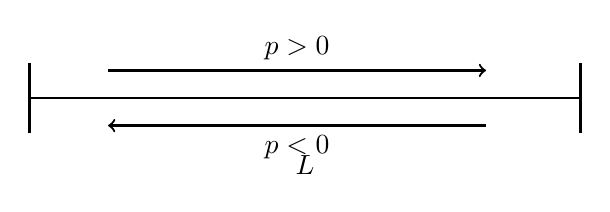
\begin{tikzpicture}[x=1cm,y=1cm]
\draw[thick] (0,0) -- (7,0);
\draw[very thick] (0,-0.45) -- (0,0.45);
\draw[very thick] (7,-0.45) -- (7,0.45);
\draw[->,thick] (1.0,0.35) -- (5.8,0.35) node[midway,above]{\(p>0\)};
\draw[->,thick] (5.8,-0.35) -- (1.0,-0.35) node[midway,below]{\(p<0\)};
\draw (3.5,-0.85) node{\(L\)};
\end{tikzpicture}
\caption{在有限线段两端处的反射使行波的动量反向。}
\end{figure}

还有一种不同的方法可以使系统有限同时保持动量守恒。将线段的两端等同起来。可以把结果画成一个圆，但不需要一个嵌入第二维中的字面意义上的圆。数学陈述很简单：坐标是周期性的：在行进总距离 \(L\) 之后，就回到同一点。

\begin{figure}[t]
\centering
\includegraphics[width=0.72\textwidth]{lecture_02_figure_06.png}
\caption{一条总长度为\(L\)的一维路径，用于引入周期性认同。}
\lectureframe{00:51:21}
\end{figure}

端点认同在下面的示意图中被明确表示出来。\footnote{该示意图遵循00处的周期性认同论证：51：09--00：52：37。}

\begin{figure}[t]
\centering
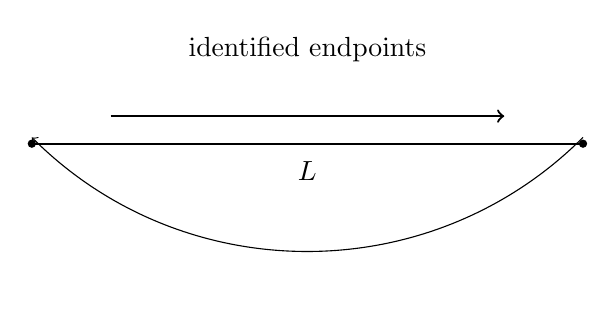
\begin{tikzpicture}[x=1cm,y=1cm]
\draw[thick] (0,0) -- (7,0);
\fill (0,0) circle (1.5pt);
\fill (7,0) circle (1.5pt);
\draw[->,thick] (1.0,0.35) -- (6.0,0.35);
\draw (3.5,-0.35) node{\(L\)};
\draw[->,bend left=45] (7,0.08) to (0,0.08);
\draw (3.5,1.2) node{identified endpoints};
\end{tikzpicture}
\caption{通过认同长度为\(L\)的路径的端点而形成的周期性一维空间。}
\end{figure}

向右运动的波随后到达所示端点，在起点处重新出现，并继续向右运动。向左运动的波同样继续向左运动。不存在波在其处反射的特定端点，因此动量不会反向。周期性空间使体积有限并保持动量，但它有一个重要后果：允许的动量是离散的。

整数个波长必须容纳在总长度之内。对于非常数模式，
\begin{equation}
\lambda_{|N|}=\frac{L}{|N|},
\qquad |N|=1,2,3,\ldots .
\end{equation}
因此波长大小可以是\(L\)、\(L/2\)、\(L/3\)，等等。诸如\(L/\sqrt{2}\)这样的选择并不适合：绕行一周后，波将以错误的相位返回，无法与其起始值匹配。

利用\(p=h/\lambda\)，第\(|N|\)个非常数模式的动量大小为
\begin{equation}
|p_N|=\frac{|N|h}{L}.
\end{equation}
为了无歧义地同时包含两个方向和常数模式，方便的做法是让模式标签带符号：
\begin{equation}
p_N=\frac{Nh}{L},
\qquad N=0,\pm1,\pm2,\ldots .
\end{equation}
正的和负的\(N\)描述相反的传播方向。\(N=0\)模式是常数模式，动量为零；它没有有限波长可供代入\(h/\lambda\)。因此基本动量间隔为\(h/L\)。

对于宏观的\(L\)，\(h\)和\(1/L\)都使这一间隔极其微小，因此允许值构成一个非常密集的集合，看起来几乎是连续的。然而，被约束在圆形导线上的珠子恰恰具有这种离散谱。

\begin{classroomqa}
\lecturetimestamp{00:58:27}
\audiencequestion{被量子化的是波的总动量，还是与一个周期相关联的动量？}
\lecturerresponse{该陈述适用于每个量子的动量。每个量子都具有允许的离散动量之一。因此，任何量子集合的总动量也是基本单位\(h/L\)的整数倍。}
\end{classroomqa}

\begin{classroomqa}
\lecturetimestamp{00:59:22}
\audiencequestion{为什么波绕行一周后必须回到相同的值？}
\lecturerresponse{被认同的端点是同一个物理点，因此可观测场在该处必须具有相同的值。不匹配将要求场在该点发生突然跳跃。这种不连续性在能量和动量上代价高昂；可容许的场位形是连续且周期性的。}
\end{classroomqa}

\begin{classroomqa}
\lecturetimestamp{01:00:09}
\audiencequestion{如果波被局域化为一个波包，会发生什么？}
\lecturerresponse{波包是平面波、或等价地是正弦和余弦的傅里叶和。在周期性空间中，该和只能包含离散的允许动量模式。因此，量子化陈述是关于每个可容许波包的傅里叶分量的陈述。}
\end{classroomqa}

\begin{classroomqa}
\lecturetimestamp{01:01:01}
\audiencequestion{如果周期长度\(L\)变得极其小，会有问题吗？}
\lecturerresponse{随着\(L\)减小，基本动量\(h/L\)变得非常大。在普通微观长度下并不暗示立即出现不一致，但试图将该构造推向普朗克长度尺度，预计将需要新的物理。}
\end{classroomqa}

现在把圆形图像按字面理解：一个珠子在半径为\(r\)的圆形金属丝上运动，其周长为\(L=2\pi r\)。其允许的切向动量为
\begin{equation}
p_N=\frac{Nh}{2\pi r}=\frac{N\hbar}{r}.
\end{equation}
对于在圆轨道上的非相对论粒子，角动量为\(mvr\)。由于在该情形下\(p=mv\)，因此这就是\(rp\)。表达式\(mvr\)并非相对论性的一般形式，因为此时\(p\)并不简单地等于\(mv\)，但动量乘以垂直距离仍然是正确的关系。用矢量形式表示，\footnote{讲座中首先用\(L\)表示角动量，随后注意到它与表示周期长度的\(L\)冲突，于是改变了符号。这里通篇使用\(J\)；参见01：03：40--01：05：21。}
\begin{equation}
\vec J=\vec r\times\vec p,
\end{equation}
而对于切向圆周运动，其大小为\(J=rp\)。因此
\begin{equation}
J_N=rp_N=N\hbar.
\end{equation}
线动量的间距取决于圆的大小，而角动量单位始终是\(\hbar\)。当涉及费米子时，整数规则存在例外；这些例外将推迟讨论。

下一项任务是把场与粒子、量子更精确地联系起来。这需要简短地回到算符和简谐振子的量子力学。

\section{波模式与量子算符}

接下来的量子力学必然是抽象的，意在作为复习。简谐振子是本质的系统，因为波就是一种振荡。在固定点上，电场、磁场或任何其他波幅都随时间周期性地变化；说一个分量具有频率，就已经是在说它振荡。

一般的波不必只具有一个波长。几种颜色的光可以混合在一起，反过来，棱镜可以把混合光分离成其组成颜色，正如牛顿对白光的分解那样。每个分量都有自己的波长、频率、振幅、能量和动量。因此，混合波可以分解为不同能量和动量的量子。每个波长决定一个频率，而每个确定频率的分量都表现为一个振子。这就是为什么简谐振子，而非任意的量子系统，是场的自然构建单元。

量子可观测量由算符表示。算符可以相加和相乘，但与普通数不同，它们的乘积不必与顺序无关。设\(A\)和\(B\)表示系统的两个性质，其中每一个本身都可能被测量。例如，\(A\)可能表示电场，而\(B\)表示磁场。如果测量值是普通数\(a\)和\(b\)，那么
\begin{equation}
ab=ba.
\end{equation}
它们的数值乘积不可能依赖于乘法顺序。然而在量子力学中，相应的算符反而可能满足\(AB-BA\neq0\)。

乍看之下这似乎荒谬。如果测量电场给出一个数，测量磁场给出另一个数，那么把这两个数相乘，无论顺序如何都必须给出相同的结果。解决之道在于，当算符乘积依赖于顺序时，这两个量就不能同时被测量。测量其中一个的实验会干扰对另一个的测量。这里没有矛盾，因为这两个数值无法同时获得。

当两个量可以同时测量时，它们的测量值是普通数，而这些数是对易的。因此，同时可测量性的检验就是对易子
\begin{equation}
[A,B]=AB-BA.
\end{equation}
对易子为零意味着可观测量相容；对易子非零意味着相应的测量相互干扰。交换两个位置会改变符号：
\begin{equation}
[B,A]=-[A,B].
\end{equation}

对于非相对论粒子，三个位置分量彼此对易，三个动量分量也彼此对易：
\begin{align}
[x,y]&=[y,z]=[z,x]=0,\\
[p_x,p_y]&=[p_y,p_z]=[p_z,p_x]=0.
\end{align}
所有三个坐标可以一起确定，所有三个动量分量也可以一起确定。相应的位置和动量分量则不对易：
\begin{equation}
[x,p_x]=[y,p_y]=[z,p_z]=i\hbar,
\end{equation}
而诸如\([x,p_y]\)这样的混合分量则为零。测量一个位置坐标会给粒子带来共轭动量上的扰动。等价地说，相应的位置和动量不确定度的乘积由\(\hbar\)控制。

\begin{classroomqa}
\lecturetimestamp{01:16:30}
\audiencequestion{当从\(x\)变到\(y\)时，对易子中的\(i\)是否应该变成\(j\)？}
\lecturerresponse{不。符号\(i\)始终是虚数单位，即负一的平方根。它既不是笛卡尔单位矢量的标记，也不是四元数符号\(i,j,k\)之一。}
\end{classroomqa}

\begin{classroomqa}
\lecturetimestamp{01:17:24}
\audiencequestion{\(AB-BA\)是否意味着先测量\(A\)，再测量\(B\)，然后颠倒测量顺序？}
\lecturerresponse{不是。这两项是不同代数次序下的算符积或矩阵积。它们并不表示字面意义上的测量序列。与不相容测量的联系是算符代数的结果，而不是该乘积的定义。}
\end{classroomqa}

\begin{classroomqa}
\lecturetimestamp{01:18:32}
\audiencequestion{这些位置--动量对易关系能直接应用于光子吗？}
\lecturerresponse{不能直接应用。它们能干净地应用于非相对论粒子。光子的位置更难定义，因此类似陈述需要更加谨慎，而这里并不需要。}
\end{classroomqa}

\section{量子谐振子}

弹簧上的重物、声波和光波都提供了振动运动的例子。每个理想谐振子都有一个频率。对于弹簧，一个完整周期不仅仅是重物回到同一位置所需的时间；它必须回到该位置并沿同一方向运动。每秒完整周期数为\(f\)，且\(\omega=2\pi f\)。

在经典情形下，理想谐振子可以具有任意非负能量。轻轻一推给出小能量，用力一推给出较大能量。真实的弹簧最终会断裂或熔化，但数学理想化具有连续的正能量范围。量子谐振子则不同：其允许的能量构成离散且等间距的阶梯。选择能量原点，使最低能级称为零，
\begin{equation}
E_n=n\hbar\omega,
\qquad n=0,1,2,\ldots .
\end{equation}
等间距能级可以如下描绘。\footnote{能级示意图遵循01处的板书讨论：21：20--01：23：56。}

\begin{figure}[t]
\centering
\begin{tikzpicture}[x=1cm,y=0.9cm]
\draw[->] (0,0) -- (0,5.35);
\draw (0,5.5) node[above]{energy};
\foreach \y/\lab in {0.6/{0},1.6/{\hbar\omega},2.6/{2\hbar\omega},3.6/{3\hbar\omega},4.6/{n\hbar\omega}}
{
  \draw[thick] (0.2,\y) -- (2.2,\y);
  \draw (-0.25,\y) node[left]{\(\lab\)};
}
\draw[->,thick] (2.8,0.68) -- (2.8,1.52);
\draw (3.2,1.1) node[right]{\(a_+\)};
\draw[->,thick] (3.7,1.52) -- (3.7,0.68);
\draw (4.1,1.1) node[right]{\(a_-\)};
\end{tikzpicture}
\caption{在约定\(E_n=n\hbar\omega\)下等间距的谐振子能级。}
\end{figure}

间距\(\hbar\omega\)与先前赋予角频率为\(\omega\)的一个光子的能量相同。数值\(2\hbar\omega\)可能属于频率为\(2\omega\)的谐振子的一个量子的能量，也可能属于频率为\(\omega\)的谐振子的两个量子的能量。这里需要的是第二种解释。一个固定频率的单一谐振子可以包含零个、一个、两个、三个或更多量子，而各阶梯之间没有允许的能量。

整数\(n\)标记谐振子态，写作右矢\(|n\rangle\)。态\(|0\rangle\)是基态，\(|1\rangle\)有一个激发量子，\(|2\rangle\)有两个，依此类推。右矢只是算符所作用状态的记号。

定义使态上升一个能级的升算符\(a_+\)和使态下降一个能级的降算符\(a_-\)：
\begin{align}
a_+|n\rangle &= \sqrt{n+1}\,|n+1\rangle,\\
a_-|n\rangle &= \sqrt{n}\,|n-1\rangle.
\end{align}
数值平方根因子是定义的一部分。作用于最低态时，
\begin{equation}
a_-|0\rangle=0,
\end{equation}
因为基态之下没有态。

这里重要的是区分普通数与算符。标记\(n\)以及诸如\(\sqrt n\)的系数是普通数；它们与一切对易。符号\(a_+\)和\(a_-\)是算符，其顺序必须保持。

先降低\(|n\rangle\)，然后再升高它。降低步骤给出
\begin{equation}
a_-|n\rangle=\sqrt n\,|n-1\rangle.
\end{equation}
用\(a_+\)作用于所得态会再提供一个因子\(\sqrt n\)，因为升高\(|n-1\rangle\)会将其送回\(|n\rangle\)：
\begin{align}
a_+a_-|n\rangle
&=a_+\bigl(\sqrt n\,|n-1\rangle\bigr)\\
&=\sqrt n\,\sqrt n\,|n\rangle\\
&=n|n\rangle.
\end{align}
因此\(a_+a_-\)读取能级数。例如，假设已知\(|\chi\rangle\)是数本征态，但其能级标记未知。如果
\begin{equation}
a_+a_-|\chi\rangle=q|\chi\rangle,
\end{equation}
那么普通数值系数\(q\)就是该态中的量子数。因此该乘积是数算符，
\begin{equation}
\hat n=a_+a_-,
\end{equation}
并且，在所选能量约定下，哈密顿量为
\begin{equation}
H=\hbar\omega\,a_+a_-.
\end{equation}
确实，作用于任意能级都给出\(H|n\rangle=n\hbar\omega|n\rangle\)。

现在颠倒顺序。先升高给出\(\sqrt{n+1}|n+1\rangle\)。随后降低返回\(|n\rangle\)，并提供第二个因子\(\sqrt{n+1}\)：
\begin{align}
a_-a_+|n\rangle
&=a_-\bigl(\sqrt{n+1}\,|n+1\rangle\bigr)\\
&=\sqrt{n+1}\,\sqrt{n+1}\,|n\rangle\\
&=(n+1)|n\rangle.
\end{align}
两种顺序在每个态上相差一，因此
\begin{equation}
[a_-,a_+]=a_-a_+-a_+a_-=1.
\end{equation}

振子还具有振幅和相位。它的相位规定了它处于循环中的哪个位置；具体而言，它可由振子沿选定方向通过原点的时间来确定。延迟该穿越会改变相位而不改变频率。阶梯算符将分别与振幅和相位相关的量子变量组合起来。它们的代数本质上是量子的，但其作用很简单：\(a_+\) 增加一个振子能量量子，\(a_-\) 减少一个。对于电磁模式，这些量子就是光子，因此这两个算符被称为产生算符和湮灭算符。

\begin{classroomqa}
\lecturetimestamp{01:37:34}
\audiencequestion{升算符和降算符是否对应于一种物理测量？}
\lecturerresponse{光子数是可测量的。算符 \(a_+\) 和 \(a_-\) 由于额外的技术原因，并非各自单独可测量的可观测量。它们的对易子表明二者不对易，但这一事实本身并不是其中任何一个单独不可观测的论据。}
\end{classroomqa}

具有不同固有频率的一组弹簧给出许多独立的振子。空腔的电磁模式也是如此：一个波长可以被激发，而不要求其他波长具有相同的激发。在量子力学中，产生算符和湮灭算符在每个独立振子中增加和减少固定频率的量子。这种语言是核心的，因为粒子将被等同于正是这些量子。

\section{场作为振子的集合}

回到总长度为 \(L\) 的周期性一维空间。其非常数模式具有波长大小
\begin{equation}
\lambda_N=\frac{L}{N},
\qquad N=1,2,3,\ldots ,
\end{equation}
以及相应的非负角频率 \(\omega_N\)。为了与先前的动量谱进行比较，将其带符号整数重新标记为 \(M\) 是有用的：
\begin{equation}
p_M=\frac{Mh}{L},
\qquad M=0,\pm1,\pm2,\ldots .
\end{equation}
\(M\) 的符号记录了传播方向。
\editorialnote{在 01：42：08--01：42：24 处，频率模式索引从带符号范围修正为从零向上延伸的范围。符号 \(M\) 在此仅用于将带符号动量记号与非负频率模式标签 \(N\) 区分开；它并不为 \(+M\) 和 \(-M\) 引入独立的占据数。非常数振子列表从 \(N=1\) 开始。}

每个允许的频率都表现为一个谐振子。能量可以独立地加到一个频率上，然后再加到另一个频率上。量子场的详细第一个例子推迟到下一讲，但态记号已经清楚了。将非常数模式从最长波长向上排列，写出
\begin{equation}
|n_1,n_2,n_3,\ldots\rangle,
\end{equation}
其中 \(n_N=0,1,2,\ldots\) 是频率为 \(\omega_N\) 的振子中的量子数。第一个条目说明有多少量子占据最长波长模式，第二个说明有多少量子占据下一个模式，如此无限继续下去。

弦的谐波使这一构造具体化。从基频到接下来两个谐波的进展被示意性地展示出来。\footnote{该示意图遵循 01：45：20--01：47：46 处的弦谐波讨论。}

\begin{figure}[t]
\centering
\resizebox{\linewidth}{!}{%
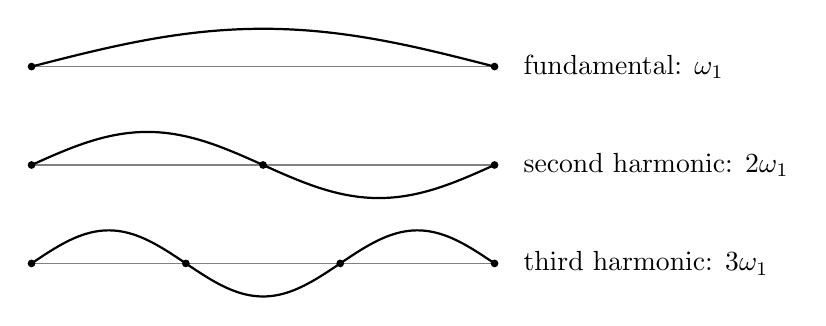
\begin{tikzpicture}[x=0.98cm,y=1cm]
\draw[gray] (0,2.5) -- (6,2.5);
\draw[thick] plot[domain=0:6,samples=120] (\x,{2.5+0.48*sin(30*\x)});
\fill (0,2.5) circle (1.4pt);
\fill (6,2.5) circle (1.4pt);
\node[right] at (6.25,2.5) {fundamental: \(\omega_1\)};

\draw[gray] (0,1.25) -- (6,1.25);
\draw[thick] plot[domain=0:6,samples=120] (\x,{1.25+0.42*sin(60*\x)});
\fill (0,1.25) circle (1.4pt);
\fill (3,1.25) circle (1.4pt);
\fill (6,1.25) circle (1.4pt);
\node[right] at (6.25,1.25) {second harmonic: \(2\omega_1\)};

\draw[gray] (0,0) -- (6,0);
\draw[thick] plot[domain=0:6,samples=120] (\x,{0.42*sin(90*\x)});
\fill (0,0) circle (1.4pt);
\fill (2,0) circle (1.4pt);
\fill (4,0) circle (1.4pt);
\fill (6,0) circle (1.4pt);
\node[right] at (6.25,0) {third harmonic: \(3\omega_1\)};
\end{tikzpicture}%
}
\caption{弦的基频及其第二和第三谐波，分别具有零个、一个和两个内部节点。}
\end{figure}

基频作为一个宽大的拱形运动，没有内部节点。它是一个振子，可以包含 \(n_1=0,1,2,\ldots\) 个量子；每次激发花费 \(\hbar\omega_1\)。第二谐波有一个内部节点，频率是基频的两倍。如果基频发出中央C，这个模式发出高一个八度的C。它具有独立的占据数 \(n_2\)，其每个量子花费 \(\hbar\omega_2=2\hbar\omega_1\)。第三谐波有两个内部节点，频率是基频的三倍。它有自己的独立占据数 \(n_3\)，同样可以是任何非负整数。

逐模式地，在上述使用的能量约定中，能量是占据数乘以量子能量。将这些贡献收集起来得到
\begin{equation}
E=\sum_{N=1}^{\infty} n_N\hbar\omega_N.
\end{equation}
\editorialnote{这个展示的求和是在 01：44：02--01：47：46 处分别陈述的模式能量的代数收集。}

同样的谐振子数学必须对每个场模式重复，每个独立振子有一个产生算符和一个湮灭算符。在这个第一个基本图像中，量子场就是整个振子集合及其产生--湮灭代数。

这种语言适用于粒子散射。具有确定能量和动量的量子进入实验，而具有其他能量和动量的量子则离开实验。初始粒子被湮灭算符移除；出射粒子由相应模式的产生算符插入到末态中。

\begin{classroomqa}
\lecturetimestamp{01:49:38}
\audiencequestion{同一个整数既被用来标记振子模式，又被用来计数其中的量子数吗？}
\lecturerresponse{有两个不同的整数。模式标签\(N\)标识空间图样；在弦的例子中，其节点数决定频率\(\omega_N\)。占据数\(n_N\)表明有多少个量子具有该频率。}
\end{classroomqa}
